\documentclass{beamer}

\usepackage[utf8]{inputenc}
\usepackage{default}
\usepackage{graphicx}
\usepackage{bbding}


% TODO Learn what this does
% source
% http://tex.stackexchange.com/questions/15952/layout-of-multiple-lines-footnotes
% this is a way to adjust foot note so it can be cutted into multiple lines
\makeatletter
\renewcommand\@makefntext[1]{\tiny\rightskip=25em\hskip0em\@makefnmark#1}
\makeatother

\makeatletter
\newcommand*{\rom}[1]{\expandafter\@slowromancap\romannumeral #1@}
\makeatother


% shows how to change default (blue) colours in the default beamer theme
% found here: http://joerglenhard.wordpress.com/tag/latex/
\definecolor{WaterlooRed}{RGB}{145,11,46}
\setbeamercolor{title}{fg=WaterlooRed}
\setbeamercolor{frametitle}{fg=WaterlooRed}
\setbeamercolor{structure}{fg=WaterlooRed}

% adds logo in the footer
\logo{
\includegraphics[scale=.25]{img/csuow}}

\title[]{MicroFuge: A Middleware Approach to Providing Performance Isolation in Cloud Storage Systems}
\author[Akshay Singh, Xu Cui, Benjamin Cassell, Bernard Wong and Khuzaima Daudjee]{Akshay Singh, Xu Cui, Benjamin Cassell, Bernard Wong and Khuzaima Daudjee}
\institute{
\includegraphics[scale=0.25]{img/UniversityOfWaterloo_logo_vert_rgb.png}}
\date{{\tiny\today}}

\begin{document}

\begin{frame}
  \titlepage
\end{frame}


\begin{frame}
  \frametitle{Cloud Computing}
  \begin{itemize}
  \item Cloud computing leverages economies of scale to improve resource sharing.
  \item This comes at the costs of reduce isolation between tenants.
  \end{itemize}
  \centering
  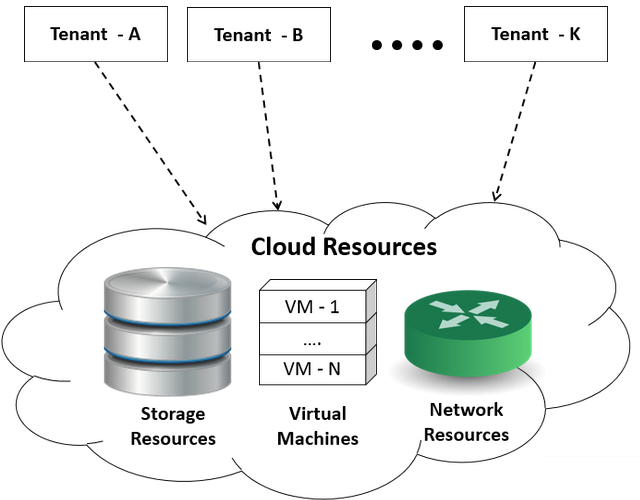
\includegraphics[scale=0.26]{img/icdcs1.png}

\end{frame}


\begin{frame}
  \frametitle{Resource Allocation in Cloud Datacenters}
  \begin{itemize}
  \item CPU - Virtualization Technologies
  \item Memory - Virtualization Technologies
  \item Network - Software Defined Networks
  \item Storage
    \begin{itemize}
    \item Virtualization Technologies degrade overall performance of the device.
    \item Cloud providers offer shared, distributed storage services.
    \item Multiple tenants: \textcolor{red}{Performance Interference}.
    \end{itemize}
  \end{itemize}
\end{frame}

\begin{frame}
  \frametitle{Typical Scenarios}
  \begin{itemize}
  \item A lot of services are backed up by cloud storage services today.
  \item Response time matters. A longer loading time can drive your customers away.
    %% \centering
    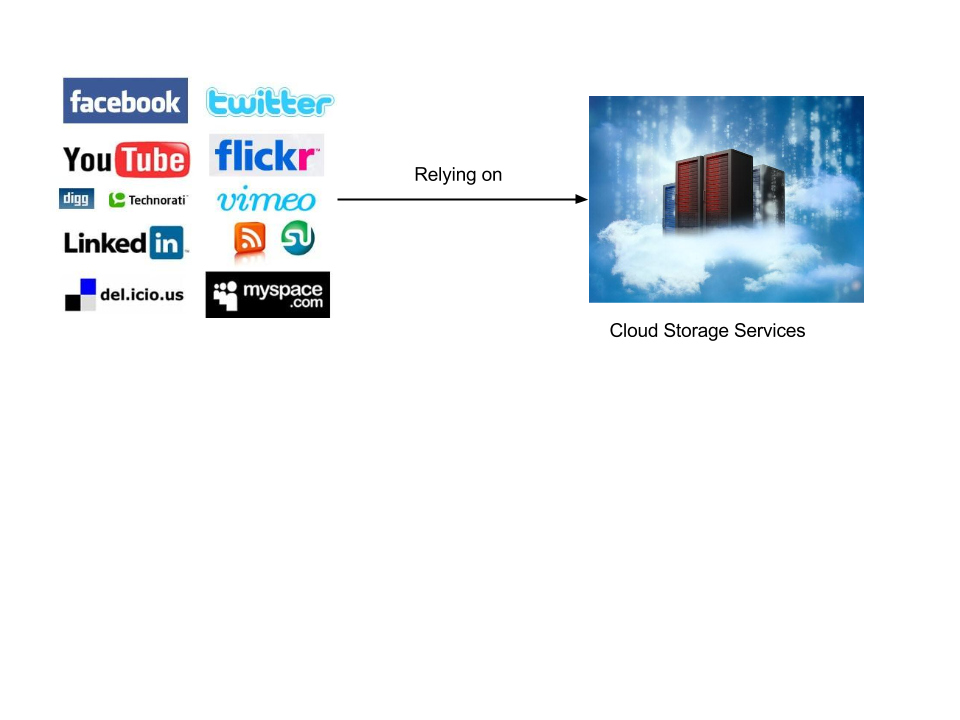
\includegraphics[scale=0.26]{img/A_Cloud_Example.png}
  \end{itemize}
\end{frame}


\begin{frame}
  \frametitle{Agenda}
  \begin{itemize}
  \item[\Checkmark] Background and Motivation
  \item MicroFuge
    \begin{itemize}
    \item Deadline Cache
    \item Deadline Scheduler
    \end{itemize}
  \item Evaluation
  \item Conclusion
  \end{itemize}
\end{frame}

\begin{frame}
  \frametitle{MicroFuge}
  \begin{itemize}
  \item A new distributed caching and scheduling middleware that provides performance isolation.
    \begin{itemize}
    \item Middleware - Reduce the barrier to adoption.
    \item Distributed - Seamlessly scalable.
    \item Multiple layers - Can be selectively adopted.
    \item Performance isolation - Relying on an empirically-driven
      performance model of the underlying storage system.
    \item Request deadlines - Model the Service Level Objectives (SLOs).
      %% model the isolation with deadlines?
    \end{itemize}
  \end{itemize}
\end {frame}


\begin{frame}
  \frametitle{Major Contributions of MicroFuge}
  \begin{itemize}
  \item \textbf{Deadline Cache (DLC)} - Deadline-aware, model-driven distributed
    caching system.
  \item \textbf{Deadline Scheduler (DLS)} - Deadline-aware distributed scheduling system.
  \item \textbf{Evaluation} - Demonstrates the effectiveness of MicroFuge in
    an EC2 deployment using the YCSB benchmark.
  \end{itemize}
\end {frame}



\begin{frame}
  \frametitle{MicroFuge at a Glance}
  \begin{itemize}
  \item MicroFuge \textit{read} operation interface.
    %% \centering
  \end{itemize}
  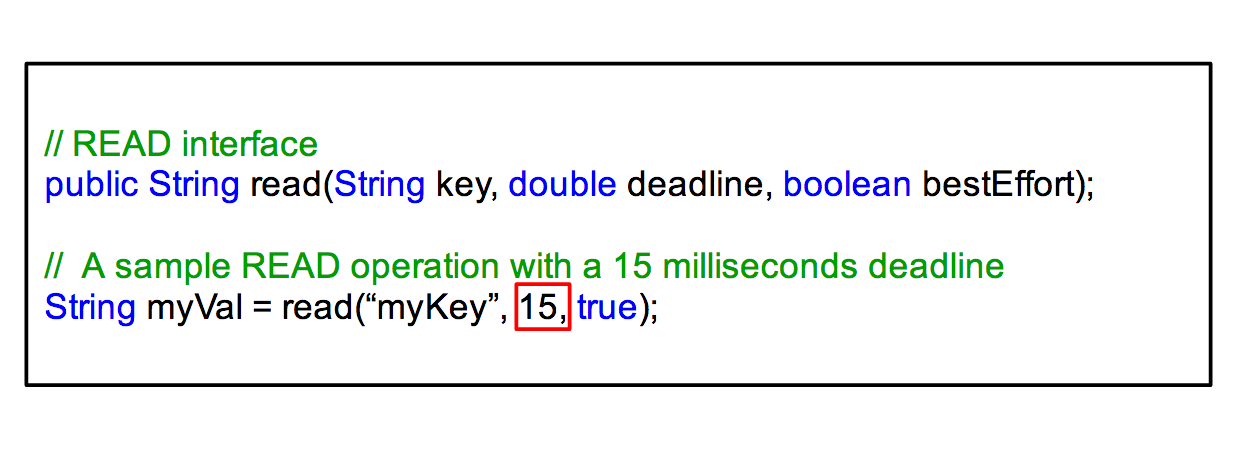
\includegraphics[scale=0.40]{img/MicroFuge_protocol.png}

\end{frame}


\begin{frame}
  \frametitle{Full MicroFuge - An example}
  \begin{itemize}
  \item Sample timeline for a read request from a client. For this request,
    the requested item is not in contained in the cache.
  \end{itemize}

  \begin{figure}
    \begin{center}
      \centerline{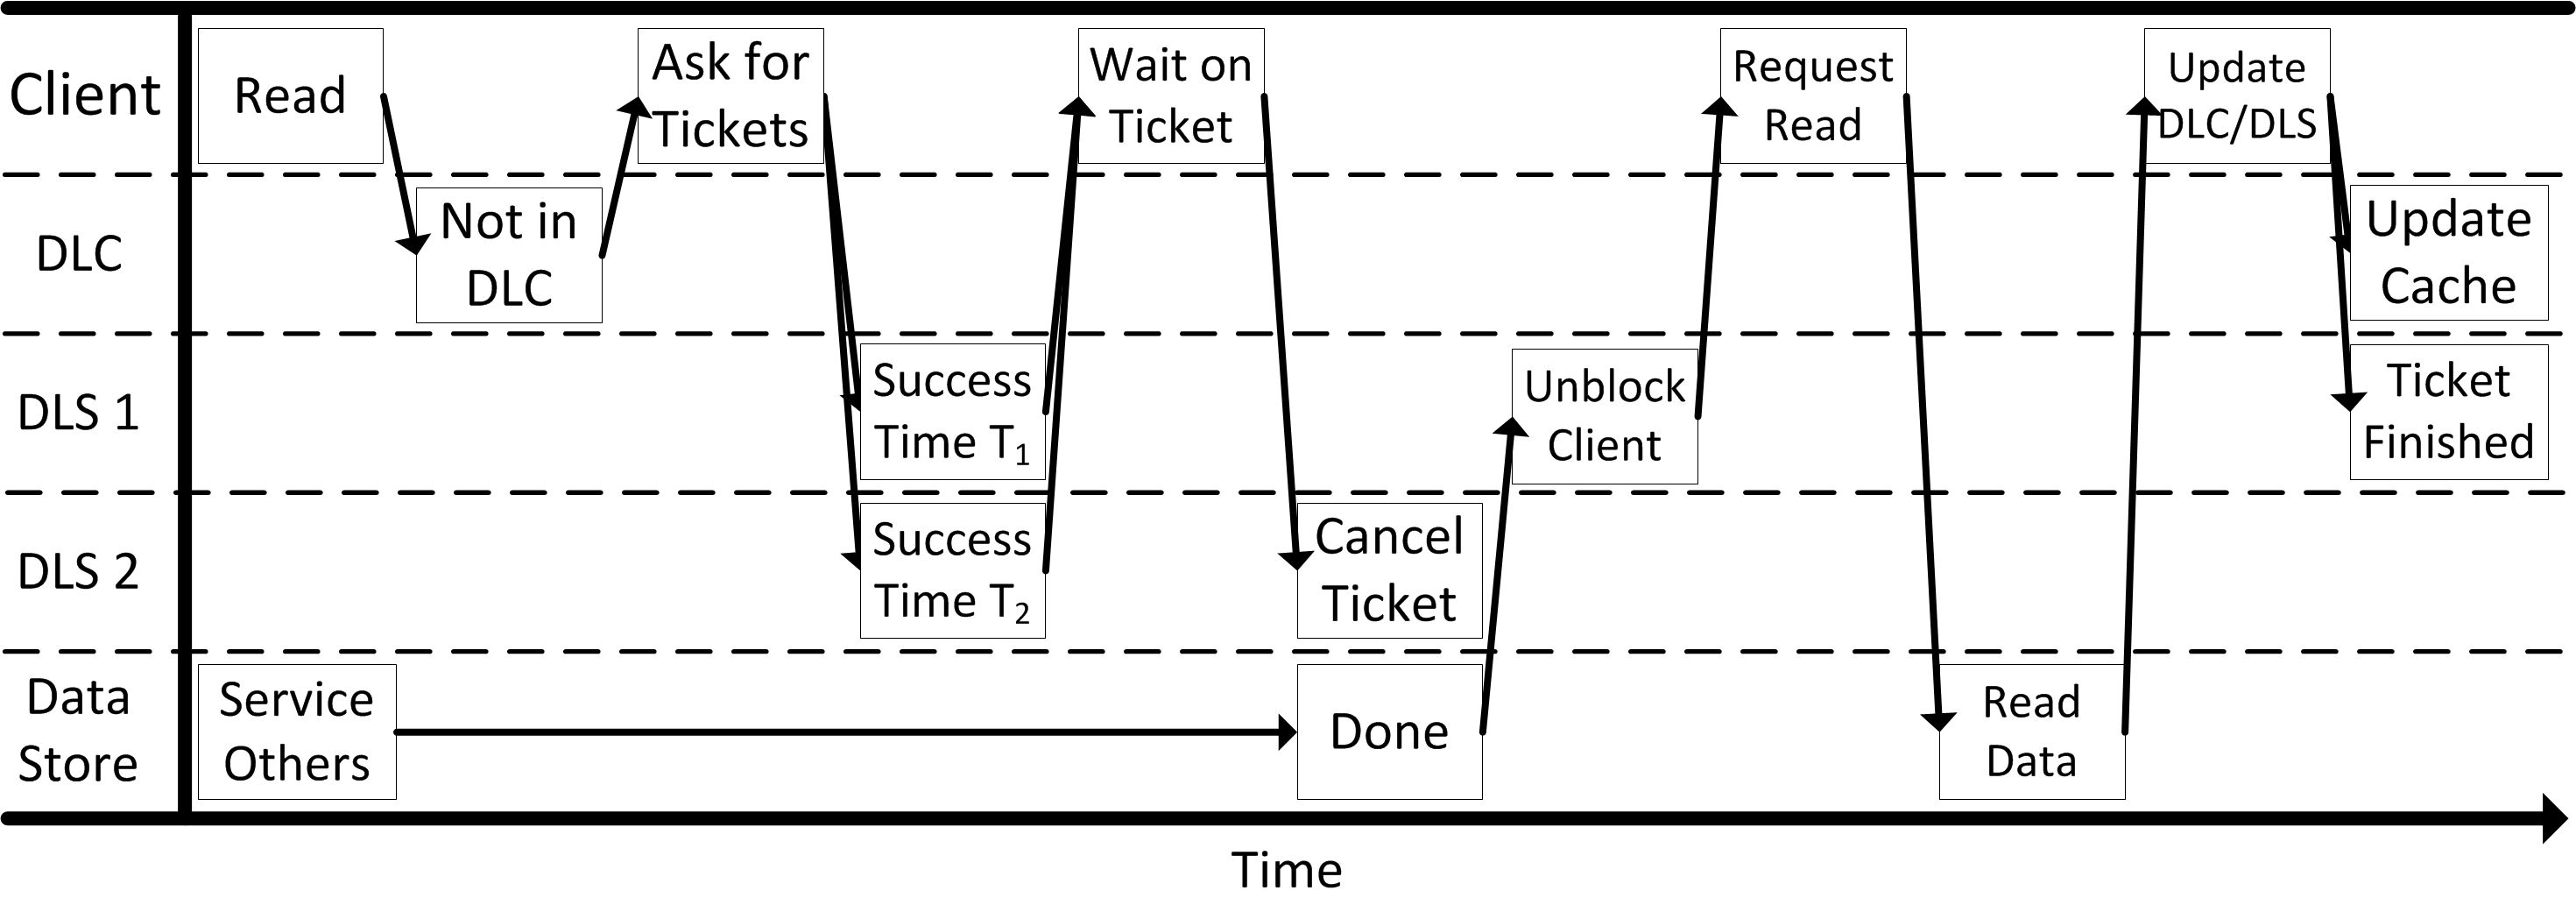
\includegraphics[scale=0.60]{img/RequestTimelineHorizontal.png}}
    \end{center}
  \end{figure}
\end {frame}

\begin{frame}
  \frametitle{Agenda}
  \begin{itemize}
  \item[\Checkmark] Background and Motivation
  \item[\Checkmark] MicroFuge
    \begin{itemize}
    \item Deadline Cache
    \item Deadline Scheduler
    \end{itemize}
  \item Evaluation
  \item Conclusion
  \end{itemize}
\end{frame}


\begin{frame}
  \frametitle{Deadline Cache (DLC) - Architecture}
  \begin{itemize}
  \item Major components - Multiple LRU queues for deadline-aware eviction and
    a performance modeling component.
  \end{itemize}
  \begin{figure}
    \begin{center}
      \centerline{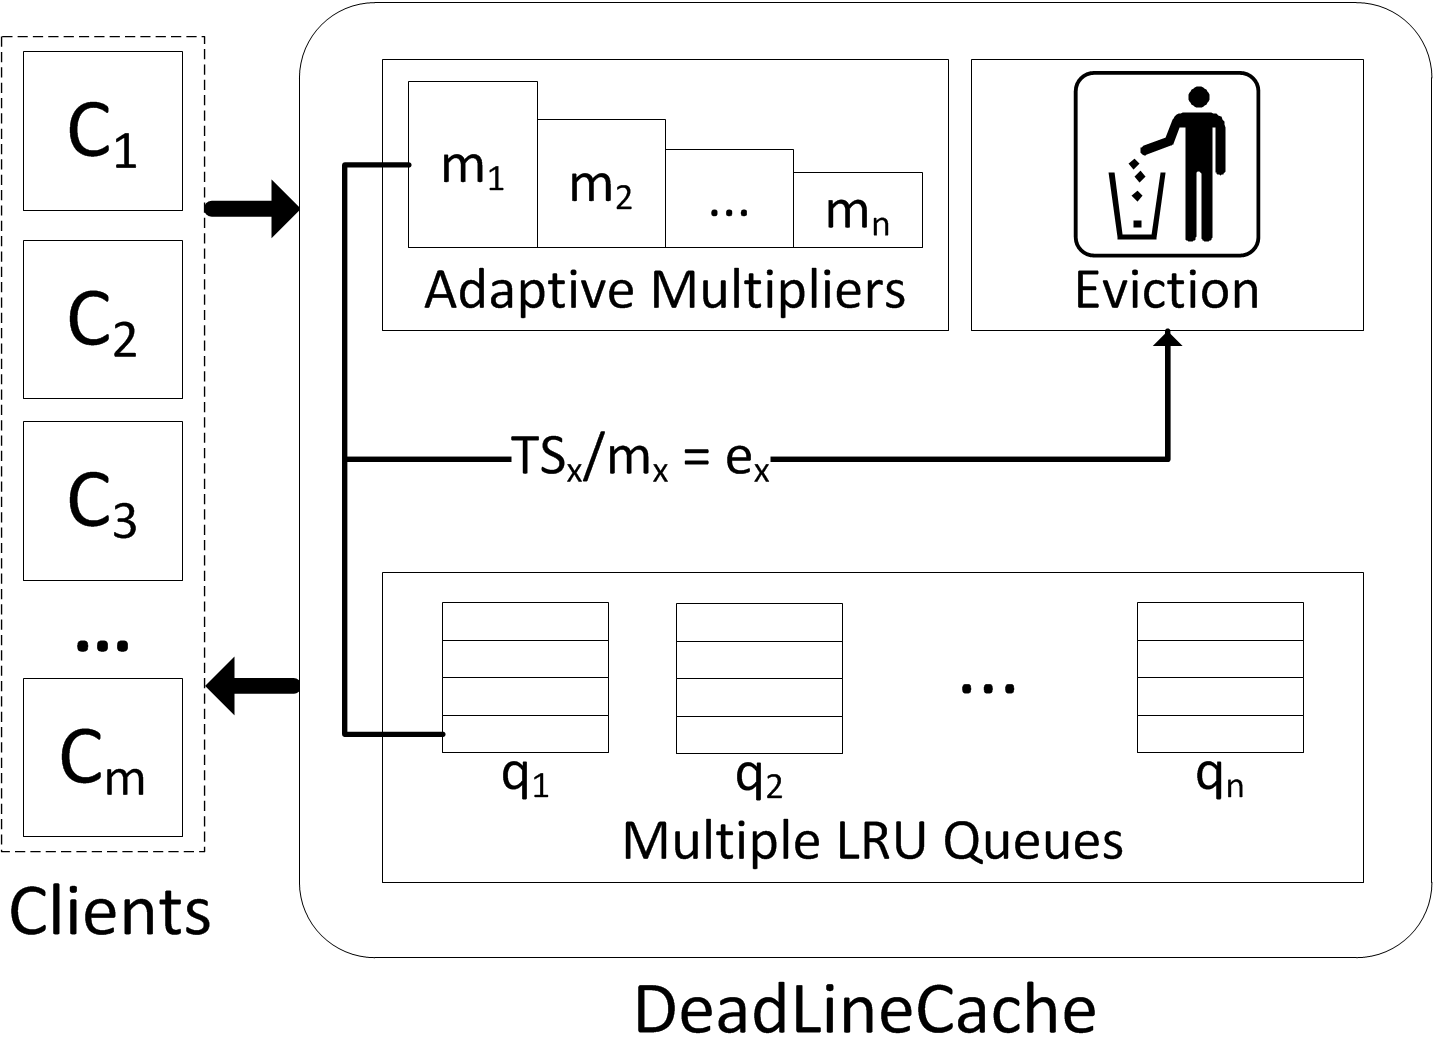
\includegraphics[scale=0.8]{img/DLC.png}}
    \end{center}
  \end{figure}
\end{frame}


\begin{frame}
  \frametitle{DLC - Adaptive Caching}
  \begin{itemize}
  \item Multiple queues - Maintain the LRU ordering of key-value pairs spanning
    different deadline ranges.
  \item Queue specific multiplier - Adaptively computed to model the likelihood
    of deadline misses within a deadline range.
  \item Modified Recency Value (MRV) - Apply the multiplier to the time elapsed
    since the last access to an item.
  \item Eviction - The item with largest MRV is evicted.
  \end{itemize}
\end{frame}


\begin{frame}
  \frametitle{DLC Interface Functions}
  \begin{itemize}
  \item Sample \textit{get, put} interface to manipulate the deadline-aware cache.
  \end{itemize}
  \begin{figure}
    \begin{center}
      \centerline{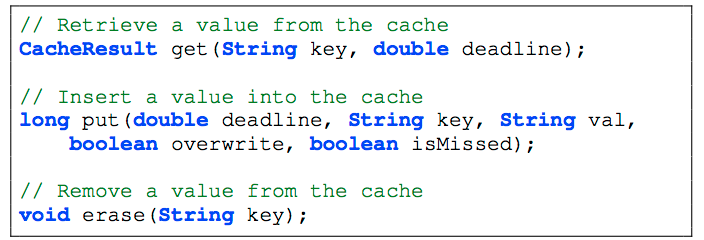
\includegraphics[scale=0.45]{img/DLC_interface.png}}
    \end{center}
  \end{figure}
\end{frame}

\begin{frame}
  \frametitle{DLC - Advantages}
  \begin{itemize}
  \item Adaptivity
    \begin{itemize}
      \item Avoids overestimating or underestimating the underlying storage
        system's performance which leads to higher deadline violations.
    \end{itemize}
  \item Easy to deploy
  \item Deadline Aware
  \end{itemize}
\end{frame}

\begin{frame}
  \frametitle{Agenda}
  \begin{itemize}
  \item[\Checkmark] Background and Motivation
  \item[\Checkmark] MicroFuge
    \begin{itemize}
    \item[\Checkmark] Deadline Cache
    \item Deadline Scheduler
    \end{itemize}
  \item Evaluation
  \item Conclusion
  \end{itemize}
\end{frame}

\begin{frame}
  \frametitle{Deadline Scheduler (DLS) High-level Architecture}
  \begin{itemize}
  \item Distributed scheduling layer - Each scheduler is responsible for
    controlling the access to a single data-server.
  \end{itemize}
  \begin{figure}
    \begin{center}
      \centerline{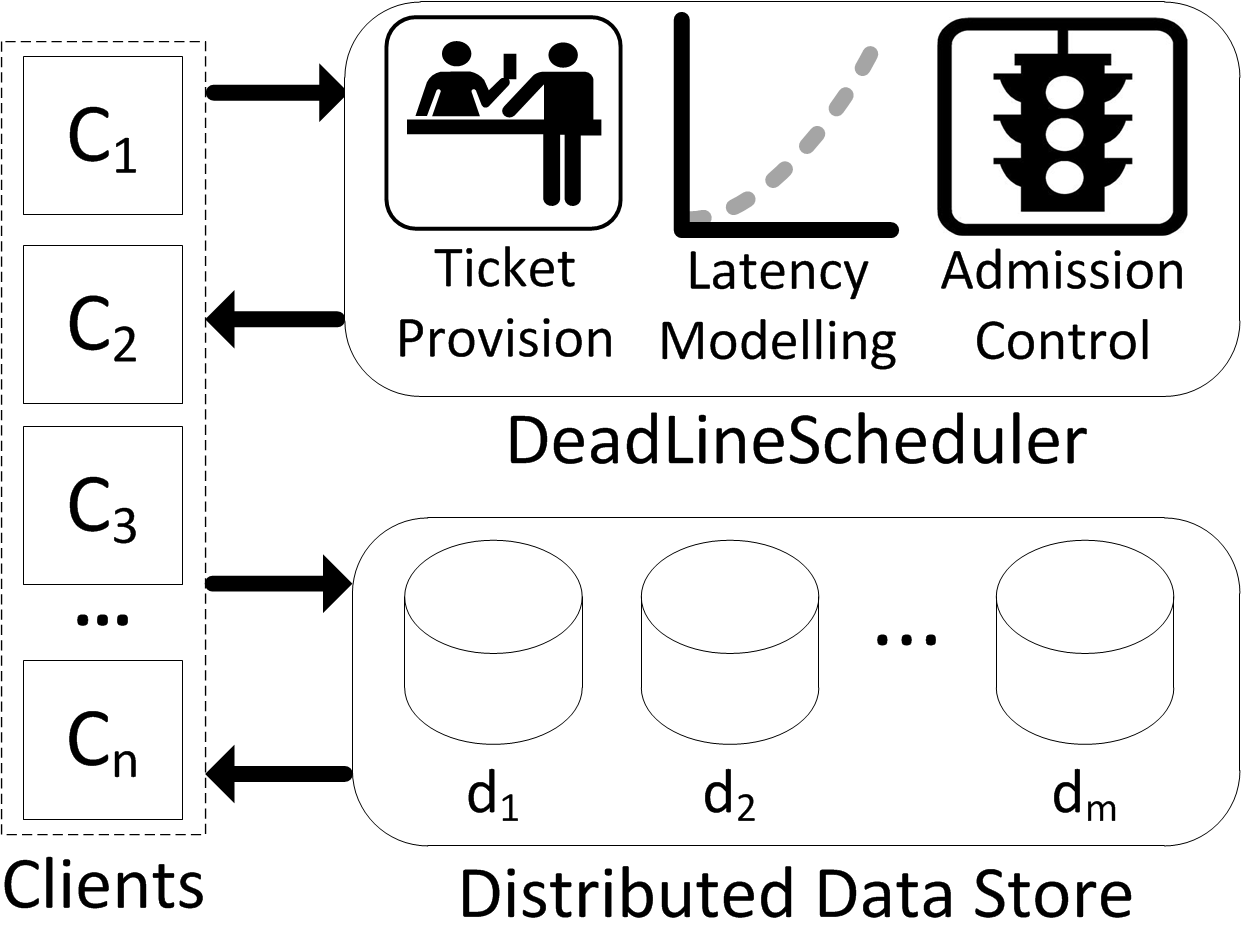
\includegraphics[scale=0.90]{img/DLS.png}}
    \end{center}
  \end{figure}
\end{frame}

\begin{frame}
  \frametitle{DLS - An Example Setup}
  \begin{itemize}
    \item Each key-value pair is replicated three times and the request issued
      by the client is best-effort.
  \end{itemize}
  \begin{figure}
    \begin{center}
      \centerline{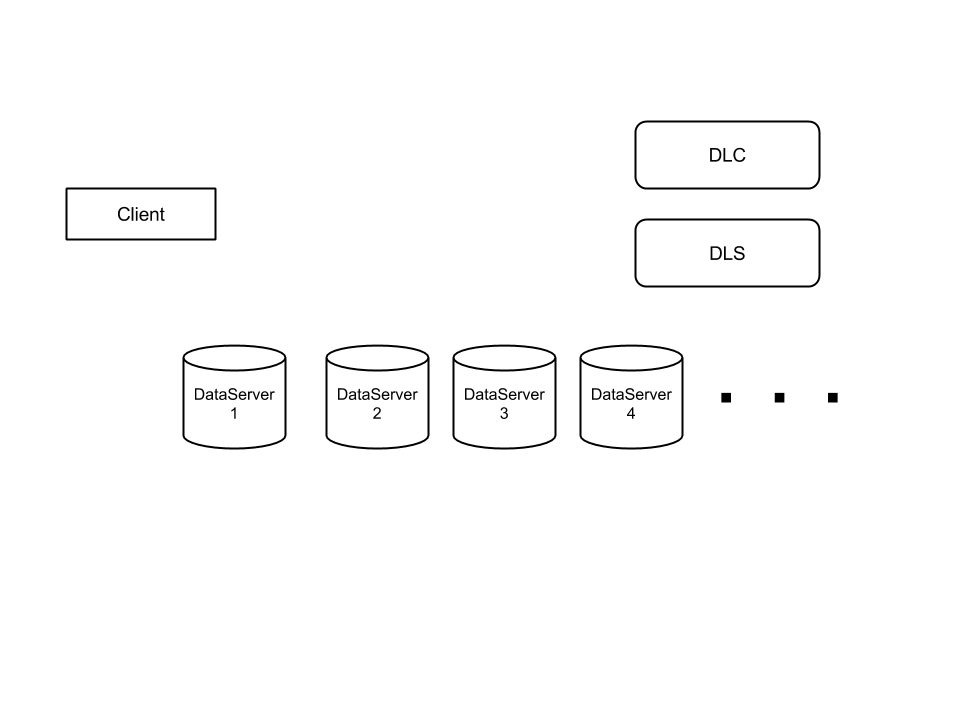
\includegraphics[scale=0.40]{img/DLS_Example1.png}}
    \end{center}
  \end{figure}
\end{frame}


\begin{frame}
  \frametitle{DLS - An Example 1}
  \begin{itemize}
    \item The client wants to perform a simple value lookup for the key UW.
  \end{itemize}
  \begin{figure}
    \begin{center}
      \centerline{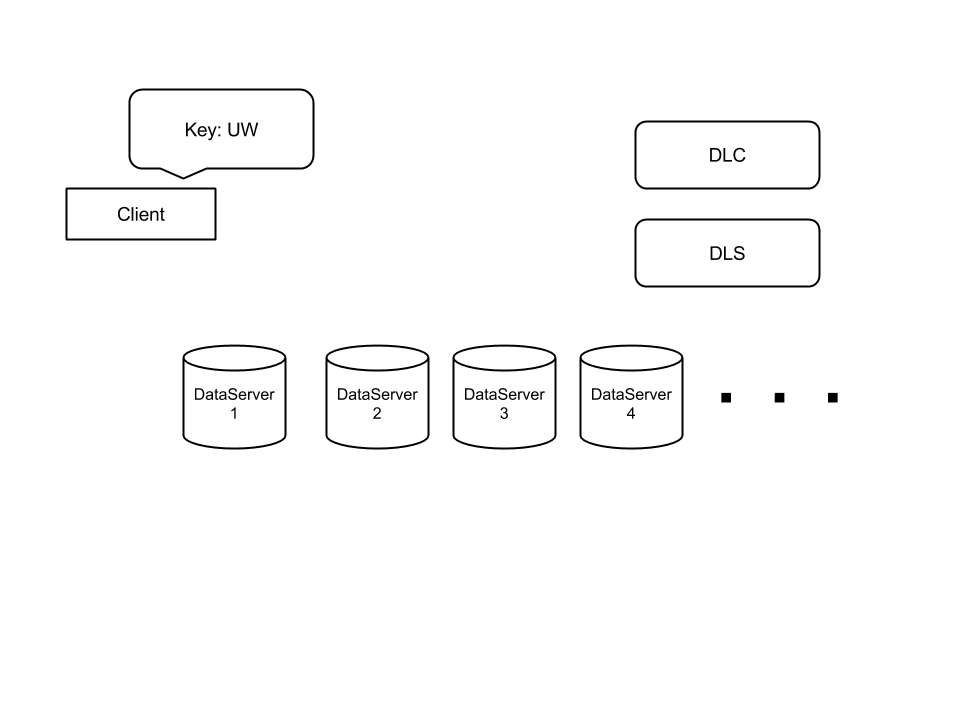
\includegraphics[scale=0.40]{img/DLS_Example2.png}}
    \end{center}
  \end{figure}
\end{frame}


\begin{frame}
  \frametitle{DLS - An Example 2}
  \begin{itemize}
    \item The client begins by issuing a cache lookup to DLC.
  \end{itemize}
  \begin{figure}
    \begin{center}
      \centerline{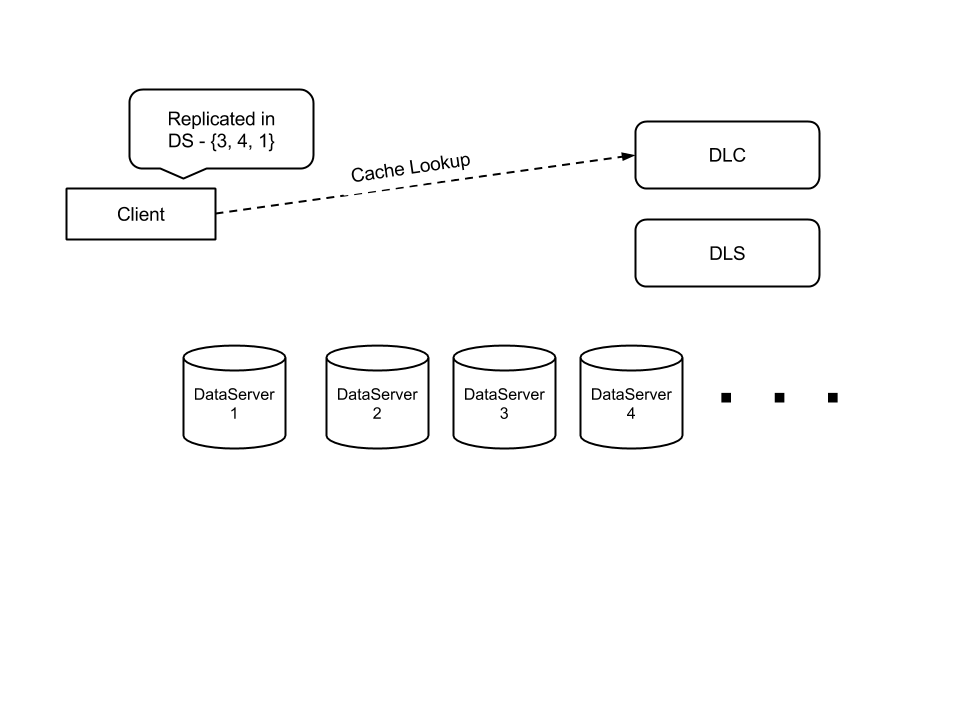
\includegraphics[scale=0.40]{img/DLS_Example3.png}}
    \end{center}
  \end{figure}
\end{frame}

\begin{frame}
  \frametitle{DLS - An Example 3}
  \begin{itemize}
    \item Concurrently, the client randomly picks two replicas and
      issue \textit{ticket get} requests to each of the replicas.
  \end{itemize}
  \begin{figure}
    \begin{center}
      \centerline{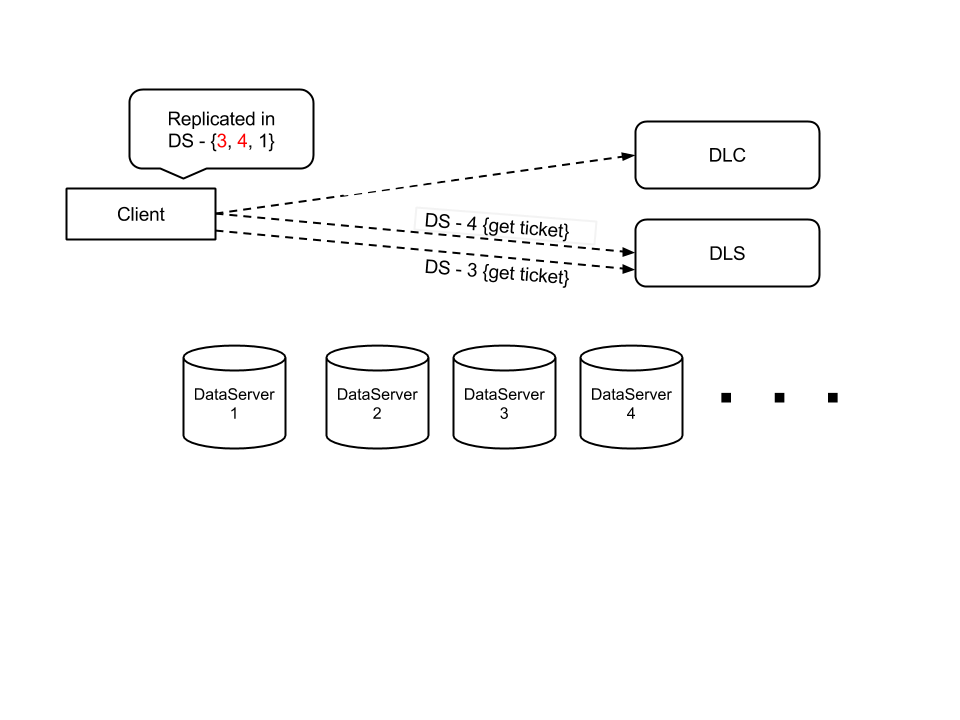
\includegraphics[scale=0.40]{img/DLS_Example4.png}}
    \end{center}
  \end{figure}
\end{frame}

\begin{frame}
  \frametitle{DLS - An Example 4}
  \begin{itemize}
    \item If the item is not in the cache, the client waits for the DLS to
      return the tickets.
  \end{itemize}
  \begin{figure}
    \begin{center}
      \centerline{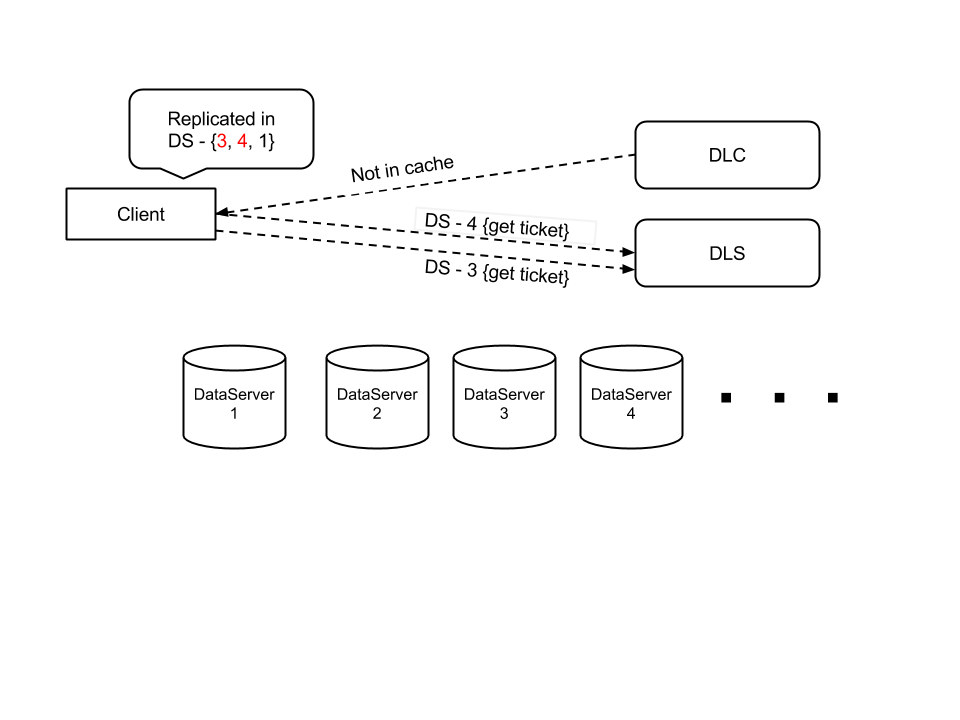
\includegraphics[scale=0.40]{img/DLS_Example5.png}}
    \end{center}
  \end{figure}
\end{frame}


\begin{frame}
  \frametitle{DLS - An Example 5}
  \begin{itemize}
    \item When the tickets are sent back to the client, the client will pick
      the DLS server which responds the first.
  \end{itemize}
  \begin{figure}
    \begin{center}
      \centerline{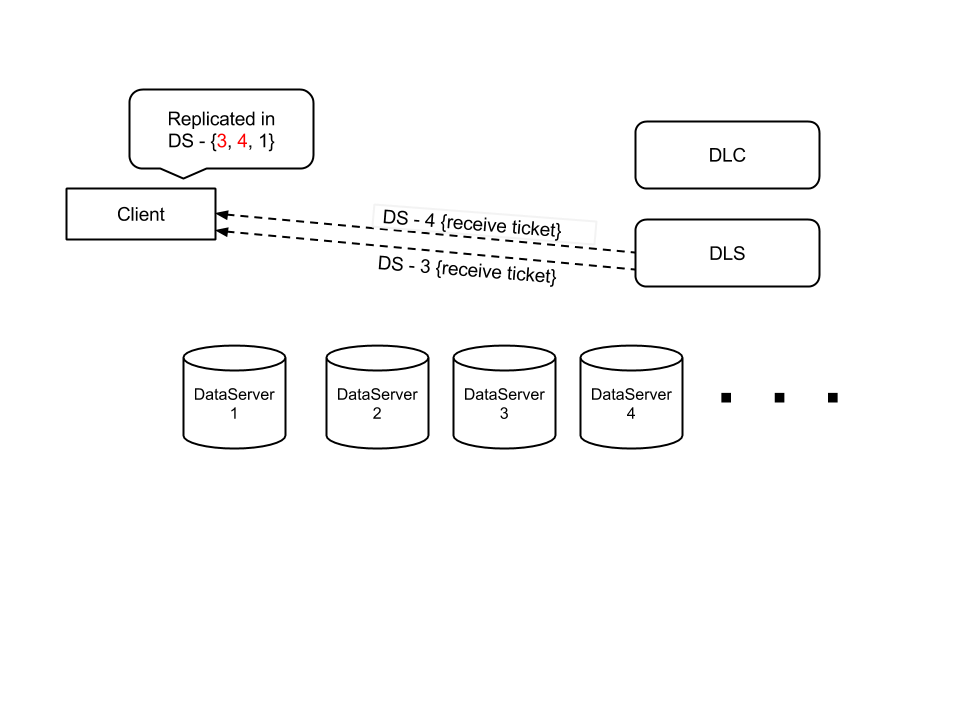
\includegraphics[scale=0.40]{img/DLS_Example6.png}}
    \end{center}
  \end{figure}
\end{frame}

\begin{frame}
  \frametitle{DLS - An Example 6}
  \begin{itemize}
    \item The client makes a blocking call to the selected DLS and waits for
      its turn to access the data server.
  \end{itemize}
  \begin{figure}
    \begin{center}
      \centerline{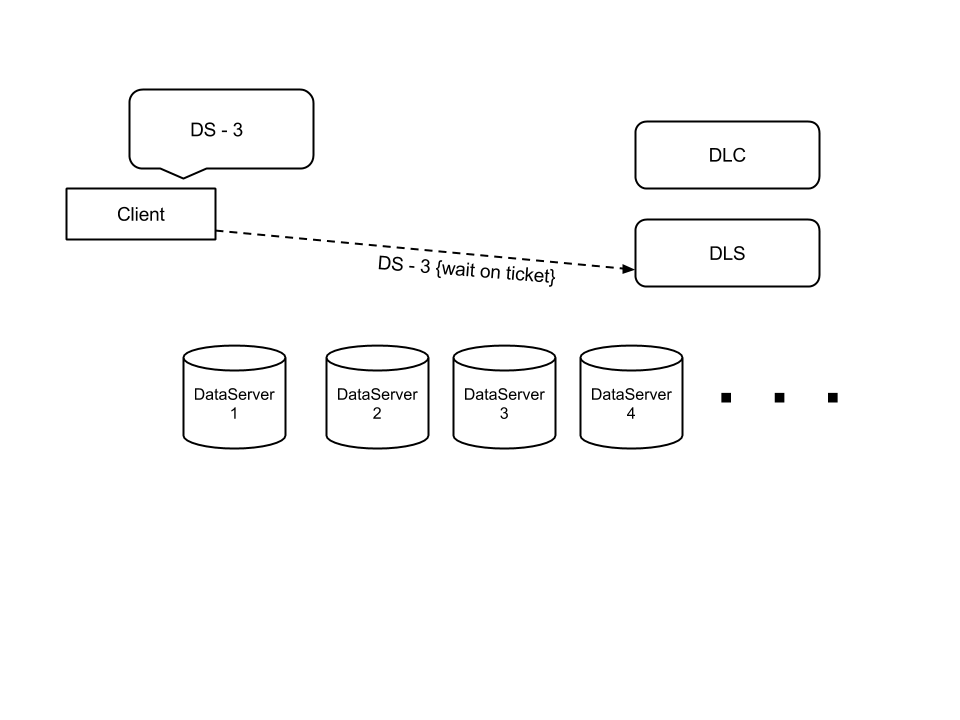
\includegraphics[scale=0.40]{img/DLS_Example7.png}}
    \end{center}
  \end{figure}
\end{frame}

\begin{frame}
  \frametitle{DLS - An Example 7}
  \begin{itemize}
    \item The client's request is inserted into DLS's pending queue.
  \end{itemize}
  \begin{figure}
    \begin{center}
      \centerline{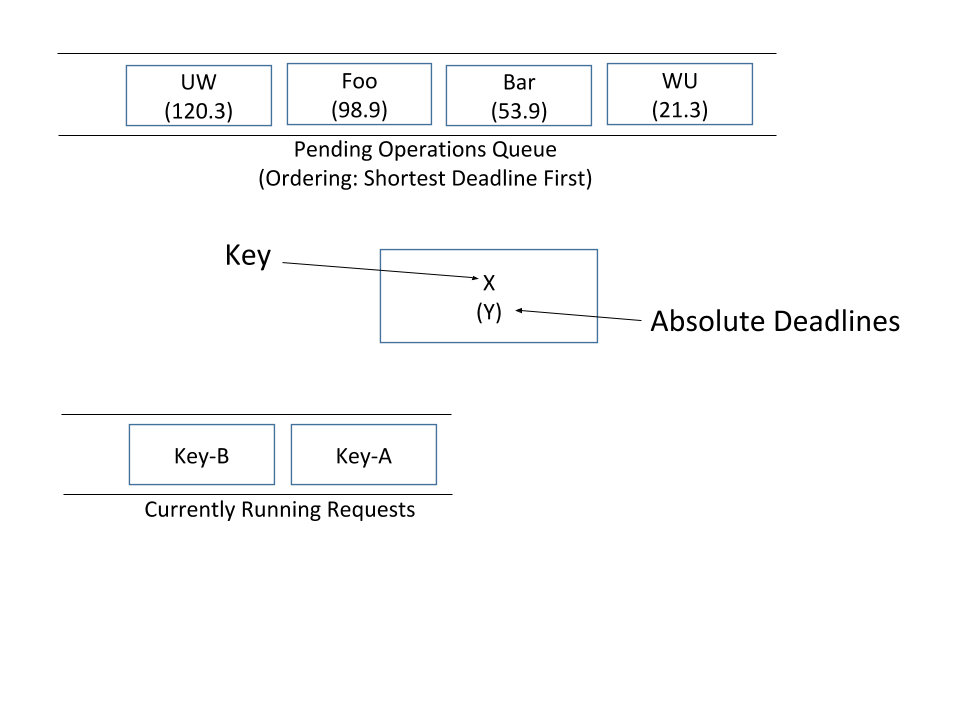
\includegraphics[scale=0.38]{img/DLS_Example8.png}}
    \end{center}
  \end{figure}
\end{frame}

\begin{frame}
  \frametitle{DLS - An Example 8}
  \begin{itemize}
    \item When a request leaves the pending queue, the DLS may increase the
      request's deadline and insert the request back into the queue if the
      deadline can not be met.
  \end{itemize}
  \begin{figure}
    \begin{center}
      \centerline{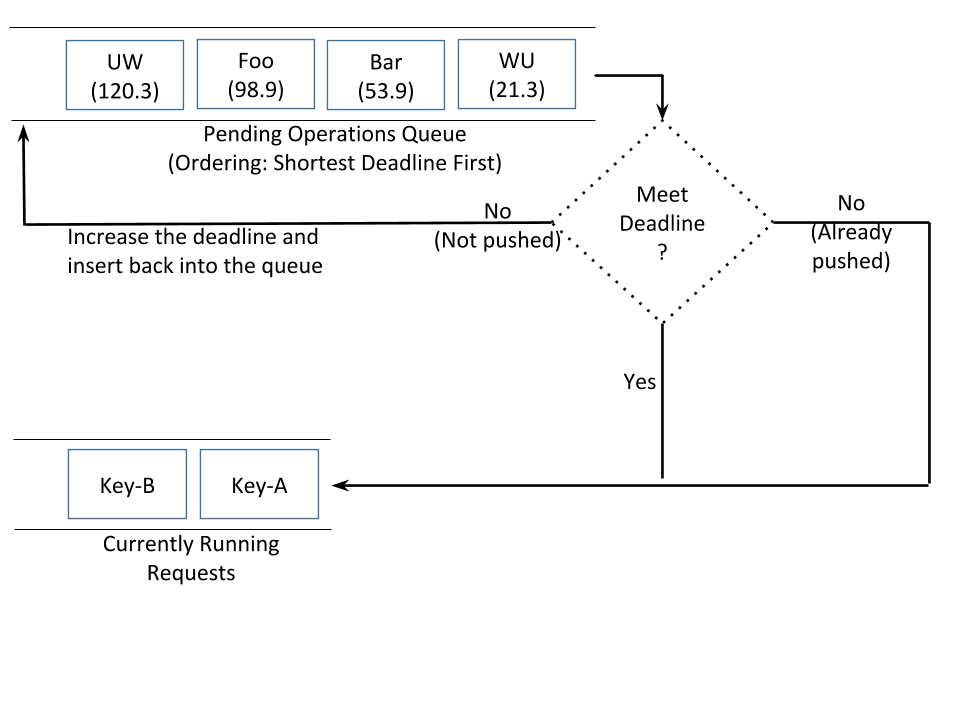
\includegraphics[scale=0.35]{img/DLS_Example9.png}}
    \end{center}
  \end{figure}
\end{frame}

\begin{frame}
  \frametitle{DLS - An Example 9}
  \begin{itemize}
  \item The DLS informs the client that the wait is over.
  \end{itemize}
  \begin{figure}
    \begin{center}
      \centerline{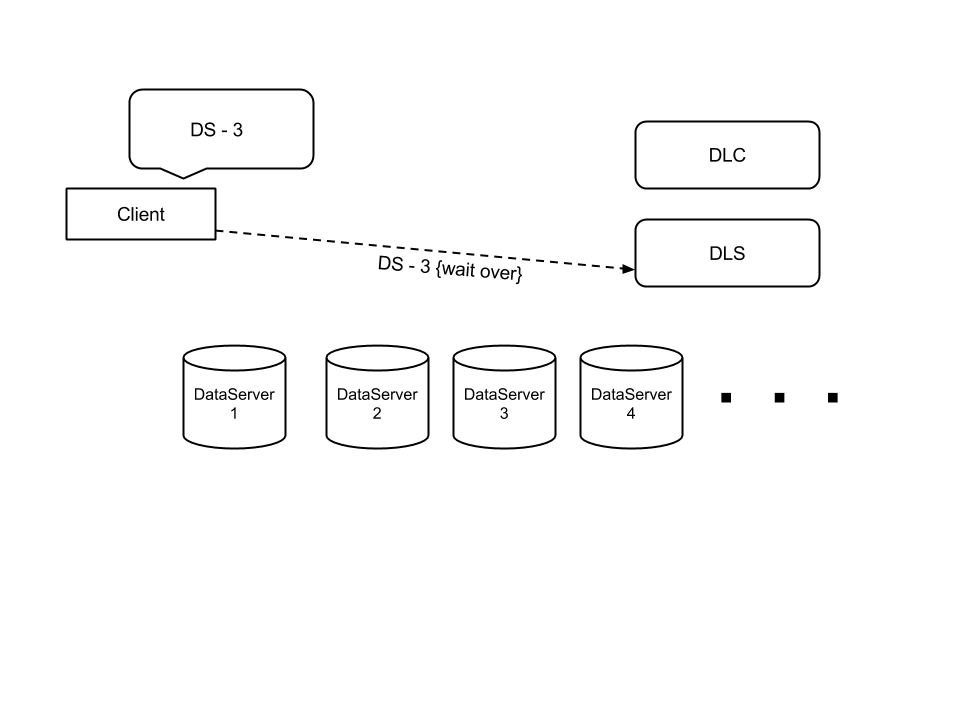
\includegraphics[scale=0.35]{img/DLS_Example10.png}}
    \end{center}
  \end{figure}
\end{frame}


\begin{frame}
  \frametitle{DLS - An Example 10}
  \begin{itemize}
  \item The clients issues the read request to the data server.
  \end{itemize}
  \begin{figure}
    \begin{center}
      \centerline{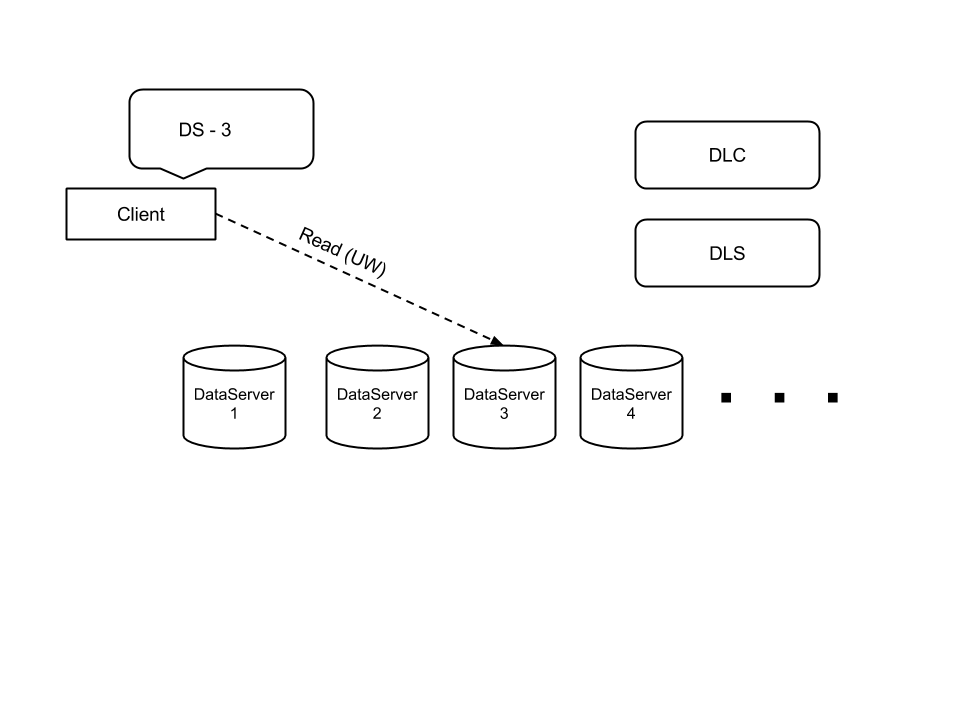
\includegraphics[scale=0.35]{img/DLS_Example11.png}}
    \end{center}
  \end{figure}
\end{frame}

\begin{frame}
  \frametitle{DLS - An Example 11}
  \begin{itemize}
  \item Upon receiving the response from the data server, the client releases
    the ticket and concurrently inserts the data into the cache.
  \end{itemize}
  \begin{figure}
    \begin{center}
      \centerline{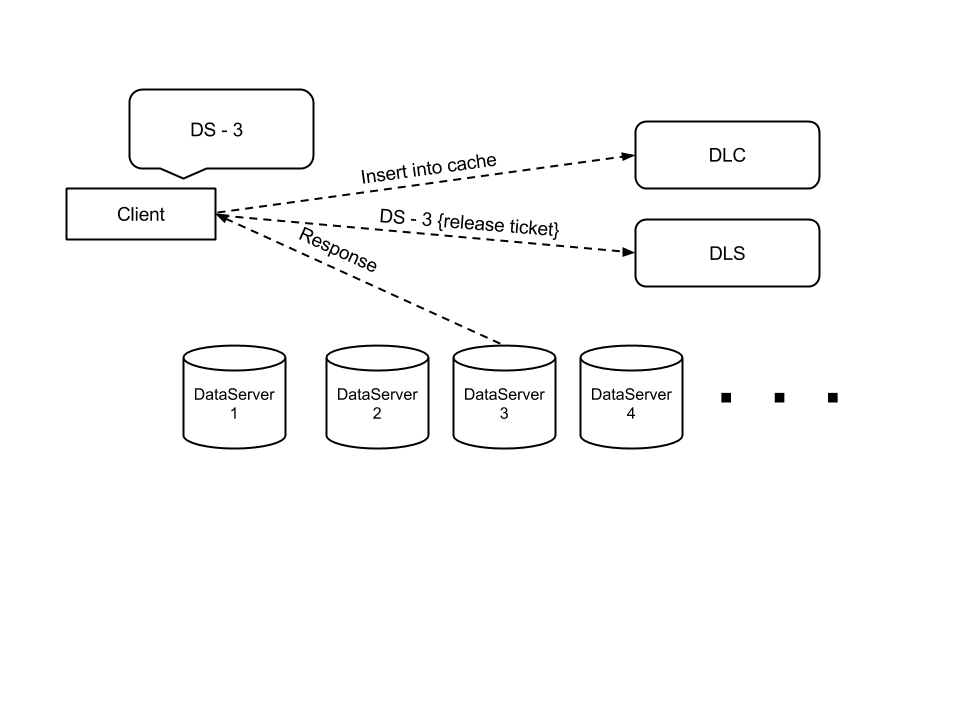
\includegraphics[scale=0.35]{img/DLS_Example12.png}}
    \end{center}
  \end{figure}
\end{frame}


\begin{frame}
  \frametitle{DLS - Admission Control}
  \begin{itemize}
  \item Bound the fraction of requests that miss their deadlines.
  \item Requests are rejected in two situations.
    \begin{itemize}
      \item The request will be miss its own deadline.
      \item The new request will cause already accepted requests to miss their deadlines.
    \end{itemize}
  \item Provides a system parameter $\beta$ as a knob to control the percentage
    of deadline misses.
  \end{itemize}
\end{frame}


\begin{frame}
  \frametitle{Agenda}
  \begin{itemize}
  \item[\Checkmark] Background and Motivation
  \item[\Checkmark] MicroFuge
    \begin{itemize}
    \item[\Checkmark] Deadline Cache
    \item[\Checkmark] Deadline Scheduler
    \end{itemize}
  \item Evaluation
  \item Conclusion
  \end{itemize}
\end{frame}

\begin{frame}
  \frametitle{Goals of the Evaluation}
  \begin{itemize}
    \item Comparison of the two caching systems.
      \begin{itemize}
        \item Deadline Cache
        \item Memcached
      \end{itemize}
    \item Effectiveness of MicroFuge.
      \begin{itemize}
      \item Caching Layer
      \item Scheduling layer
      \item Admission control
  \end{itemize}
  \end{itemize}
\end{frame}


\begin{frame}
  \frametitle{Experimental Setup - The Cluster}
  \begin{itemize}
  \item Twenty-node test cluster on AWS. Each cluster node is an m1.medium
    EC2 instance.
  \end{itemize}
  \begin{figure}
    \begin{center}
      \centerline{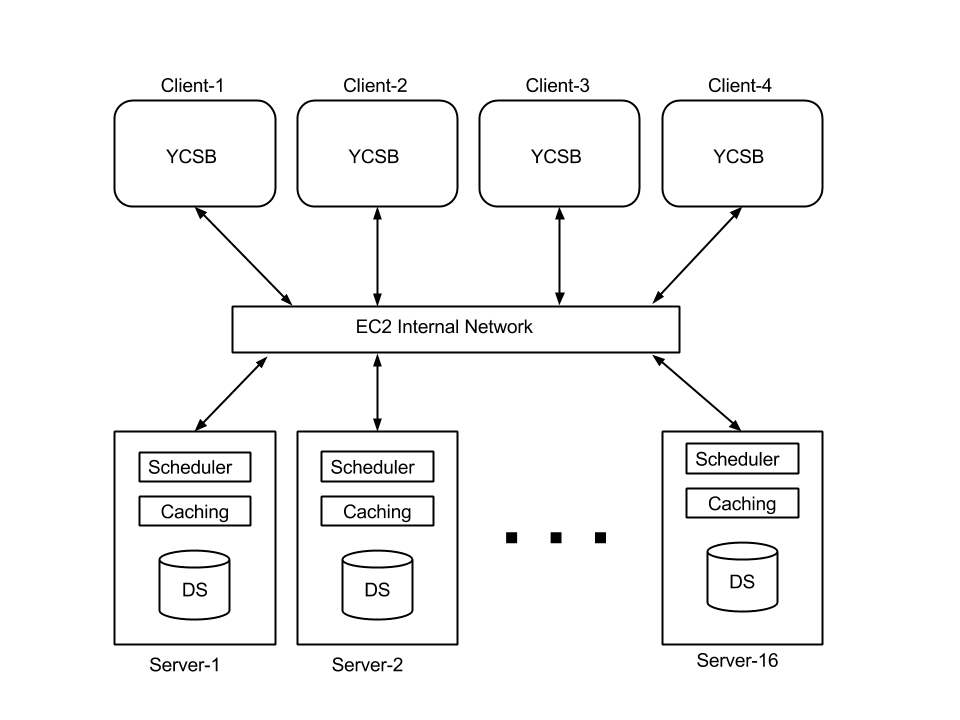
\includegraphics[scale=0.25]{img/Experimental_Setup.png}}
    \end{center}
  \end{figure}
\end{frame}

\begin{frame}
  \frametitle{Experimental Setup - Details}
  \begin{itemize}
  \item DataServer - Simple key-value store that uses leveldb with a
    replication factor 3.
  \item Benchmarking System - Modified version of Yahoo! Cloud Serving
    Benchmark (YCSB).
    \begin{itemize}
    \item Assign deadlines to each key.\\
      %% \begin{center}
      \begin{tabular}{| l | c |}
        \hline
        Range & Percentage \\ \hline
        10-30ms & 20\% \\ \hline
        30-100ms & 30\% \\ \hline
        100-1000ms & 50\% \\ \hline
      \end{tabular}
      %% \end{center}
    \end{itemize}
  \item Data Set - Key-value store with 80 million records, 86.4 GB in size.
  \item Cache - Total capacity of 19.2GB.
  \end{itemize}
\end{frame}


\begin{frame}
\frametitle{Experimental Results - Deadline-Aware Caching 1}
\begin{figure}[t]
\begin{center}
\centerline{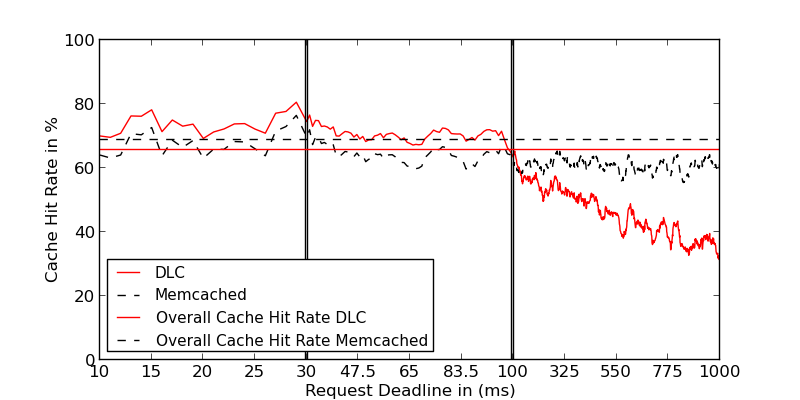
\includegraphics[scale=0.5]{img/EC2/EC2_CS_MM/cache_48.png}}
\caption{Cache hit rate for 192 concurrent clients with DLC and Memcached.}
\label{fig:cache_192_cs_mm}
\end{center}
\end{figure}
\end{frame}

\begin{frame}
\frametitle{Experimental Results - Deadline-Aware Caching 2}
\begin{figure}[t]
\begin{center}
\centerline{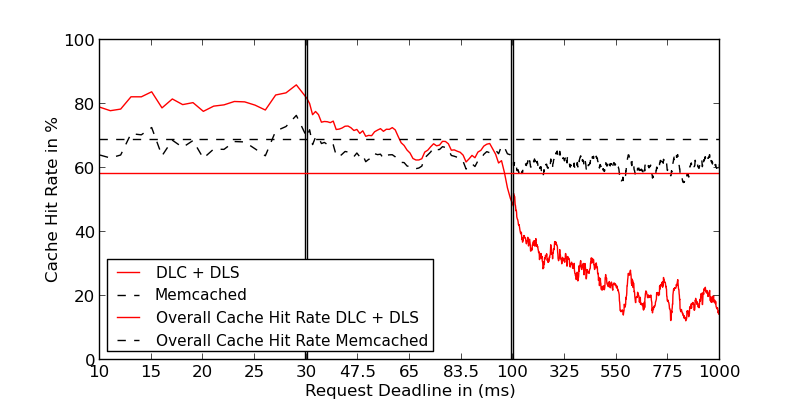
\includegraphics[scale=0.5]{img/EC2/EC2_SH_MM/cache_48.png}}
\caption{Cache hit rate for 192 concurrent clients with DLC + DLS and Memcached.}
\label{fig:cache_192_sh_mm}
\end{center}
\end{figure}
\end{frame}




\begin{frame}
  \frametitle{Experimental Results - Deadline Miss 1}
    \begin{figure}[t]
      \begin{center}
        \centerline{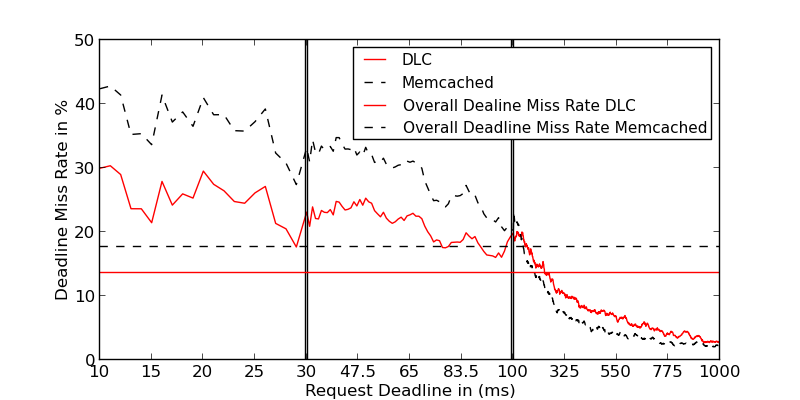
\includegraphics[scale=0.5]{img/EC2/EC2_CS_MM/miss_48.png}}
        \caption{Deadline miss rate for 192 concurrent clients with DLC and Memcached.}
        \label{fig:miss_192_cs_mm}
      \end{center}
    \end{figure}
\end{frame}


\begin{frame}
\frametitle{Experimental Results - Deadline Miss 2}
\begin{figure}[t]
\begin{center}
\centerline{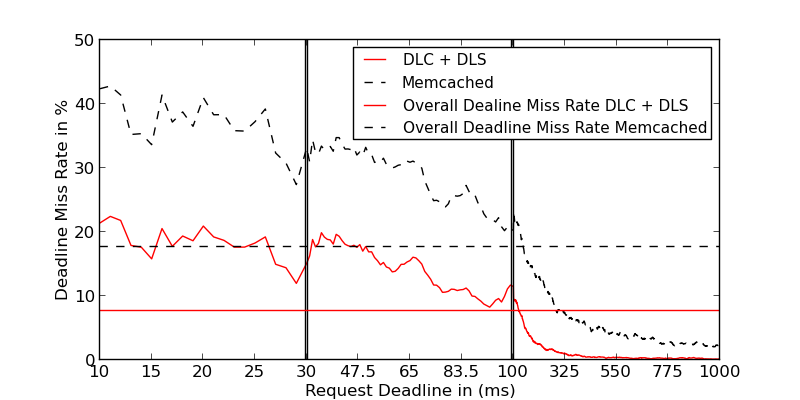
\includegraphics[scale=0.5]{img/EC2/EC2_SH_MM/miss_48.png}}
\caption{Deadline miss rate for 192 concurrent clients with DLC + DLS and Memcached.}
\label{fig:miss_192_sh_mm}
\end{center}
\end{figure}
\end{frame}

\begin{frame}
\frametitle{Experimental Results - Deadline Miss 3}
\begin{figure}[t]
\begin{center}
\centerline{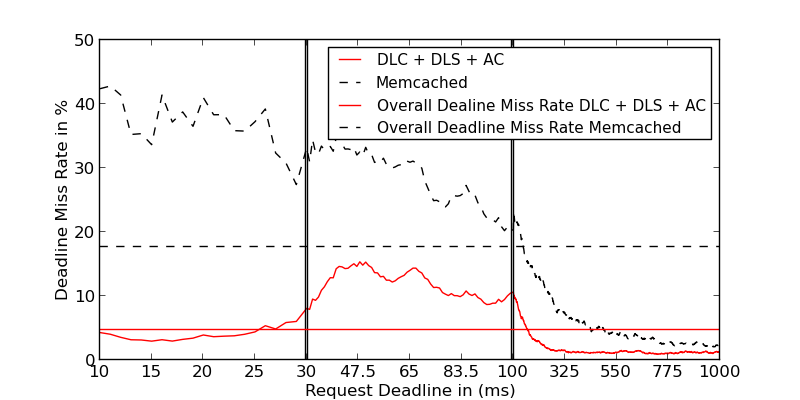
\includegraphics[scale=0.5]{img/EC2/EC2_AC_MM/miss_48.png}}
\caption{Deadline miss rate for 192 concurrent clients with DLC + DLS + AC and Memcached.}
\label{fig:miss_192_ac_mm}
\end{center}
\end{figure}
\end{frame}

\begin{frame}
\frametitle{Experimental Results - Tunable Admission Control}
\begin{figure}[t]
\begin{center}
\centerline{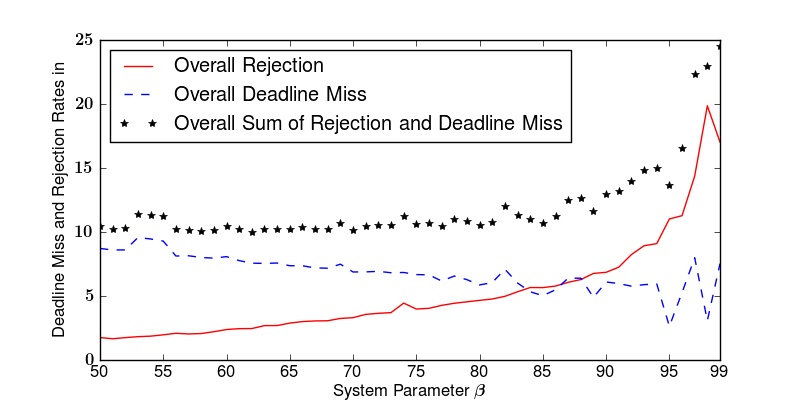
\includegraphics[scale=0.5]{img/EC2/Varying_ac/varying_acPerc_192.png}}
\caption{Deadline miss vs. rejection rates with respect to various values of
  system parameter $\beta$ for 192 clients.}
\label{fig:varying_ac}
\end{center}
\end{figure}
\end{frame}


\begin{frame}
\frametitle{Experimental Results - Overall Miss Rates}
\begin{figure}[t]
\begin{center}
\centerline{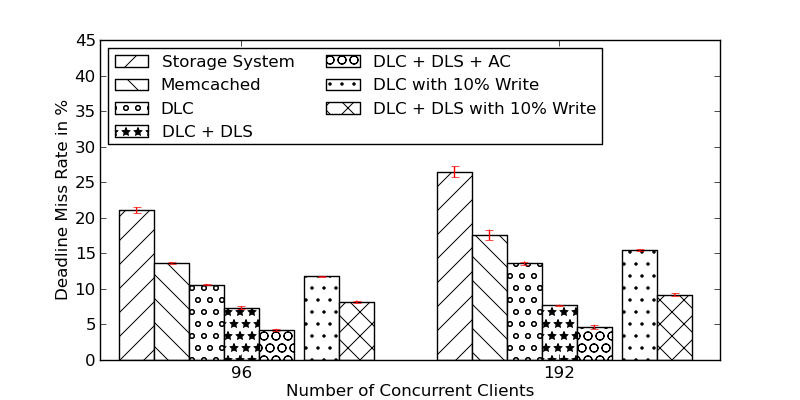
\includegraphics[scale=0.5]{img/EC2/EC2_BAR/miss_bar.png}}
\caption{Overall deadline miss rate with various system setups for
  96 and 192 concurrent clients.}
\label{fig:bar_miss}
\end{center}
\end{figure}
\end{frame}




\begin{frame}
  \frametitle{Agenda}
  \begin{itemize}
  \item[\Checkmark] Background and Motivation
  \item[\Checkmark] MicroFuge
    \begin{itemize}
    \item[\Checkmark] Deadline Cache
    \item[\Checkmark] Deadline Scheduler
    \end{itemize}
  \item[\Checkmark] Evaluation
  \item Conclusion
  \end{itemize}
\end{frame}





\begin{frame}
  \frametitle{Conclusion}
  \begin{itemize}
  \item Predictable performance is necessary in multi-tenant environments.
  \item MicroFuge - A middleware approach to performance isolation in cloud
    storage systems.
  \item Deadline awareness - Reduces deadline miss rate from over 20\% to
    less than 5\%.
  \end{itemize}
\end{frame}

\end{document}
